\chapter{Analisi}
\label{cap:analisi}

\intro{In questo capitolo si approfondisce in dettaglio il funzionamento del framework OpenVLC, le minacce alla sicurezza a cui è soggetto e le possibili contromisure.}\\

% ================================================================= %
\section{Analisi della piattaforma OpenVLC}

\paragraph{Introduzione.}
OpenVLC è una piattaforma open source per la comunicazione ottica wireless, sviluppata dal Pervasive Wireless Systems group del Dr. Giustiniano all'IMDEA Networks Institute (Madrid, Spagna).
OpenVLC è progettata per consentire agli sviluppatori di sperimentare con la \gls{vlc}, per essere flessibile e low-cost, permettendo, nell'ultima versione, la trasmissione di dati ad una velocità di 400 kb/s e ad una distanza di quasi 20 metri.

\paragraph{Motivazioni.}
Si è scelto di utlizzare OpenVLC proprio a causa della sua accessibilità e popolarità. Infatti, nonostante sia un progetto di piccole dimensioni, possiede delle caratteristiche, come ad esempio l'essere open source e l'avere una community di discrete dimensioni, che lo rendono la soluzione ideale, e probabilemente l'unica, per la ricerca in ambito \gls{vlc}.\\
È infatti importante evidenziare, che durante lo svolgimento del progetto, a causa di problematiche riscontrate nella configurazione delle due schede BeagleBone, si è valutata l'idea di trovare un'alternativa ad OpenVLC. Si è considerato, ad esempio, l'utilizzo di un software diverso o addirittura di un qualche programma che permettesse di simulare una comunicazione tramite luce visibile. Tuttavia a seguito di varie ricerche, si è concluso che OpenVLC fosse l'unica soluzione open source attualmente in circolazione.

\paragraph{Hardware.}
OpenVLC si appoggia su schede BeagleBone Black, una piattaforma hardware open source low-cost per sviluppatori, dotata di un processore ARM Cortex-A8 e di una serie di interfacce di comunicazione, tra cui USB, Ethernet e GPIO. BeagleBone è particolarmente adatta per applicazioni embedded e IoT, grazie alla sua flessibilità e alle sue capacità di elaborazione.\\
La seconda componente hardware fondamentale per il funzionamento di OpenVLC è l'\textit{OpenVLC1.3 cape}, una scheda di espansione progettata per la BeagleBone Black. Questo cape integra i circuiti necessari per la trasmissione e la ricezione di segnali luminosi, includendo un LED per l'emissione e un fotodiodo per la ricezione. Inoltre, il cape dispone di circuiti di amplificazione e filtraggio per garantire una comunicazione affidabile e ridurre il rumore di fondo. L'interfaccia tra la BeagleBone e il cape avviene tramite i pin GPIO, permettendo una gestione diretta dei segnali ottici tramite software.

\paragraph{Driver e Sistema Operativo.}
% come funziona l'ambiente di OpenVLC (descrizione ad alto livello del sistema)
Il codice sorgente di OpenVLC è formato da due componenti: il software necessario a gestire i livelli \gls{phy} e \gls{mac} e ad interfacciarli con i livelli superiori del modello \gls{osi}; il firmware necessario a controllare i \gls{pru} delle schede BeagleBone.\\
Nella versione 1.3 è stata introdotta la possibilità di utilizzare anche un LED infrarossi per trasmettere dati, il quale può affiancare il classico LED oppure essere usato singolarmente.
Di conseguenza, nel caso del trasmettitore, il framework può essere selezionato tra varie possibilità a seconda del livello di dimming desiderato. Ovvero in funzione di quanto si desidera usare il LED VL piuttosto che il LED IR.
Di seguito le possibili opzioni fornite in OpenVLC:
\begin{itemize}
    \item 0\% Dimming (solo luce visibile)
    \item 25\% Dimming
    \item 50\% Dimming
    \item 75\% Dimming
    \item 100\% Dimming (solo infrarossi)
\end{itemize}
Nell'ambito del progetto qui presentato, trattandosi di \gls{vlc}, si è deciso di usare la prima opzione, ovvero solo luce visibile.

In figura \ref{fig:beaglebone_cape} si possono osservare una scheda BeagleBone Black (a sinistra) ed un \textit{OpenVLC1.3 cape}. Sul cape \textit{IR LED} indica il LED infrarossi, \textit{VL LED} indica il LED visible light e \textit{PD} indica il fotodiodo ricevitore.
\begin{figure}[H] 
    \centering 
    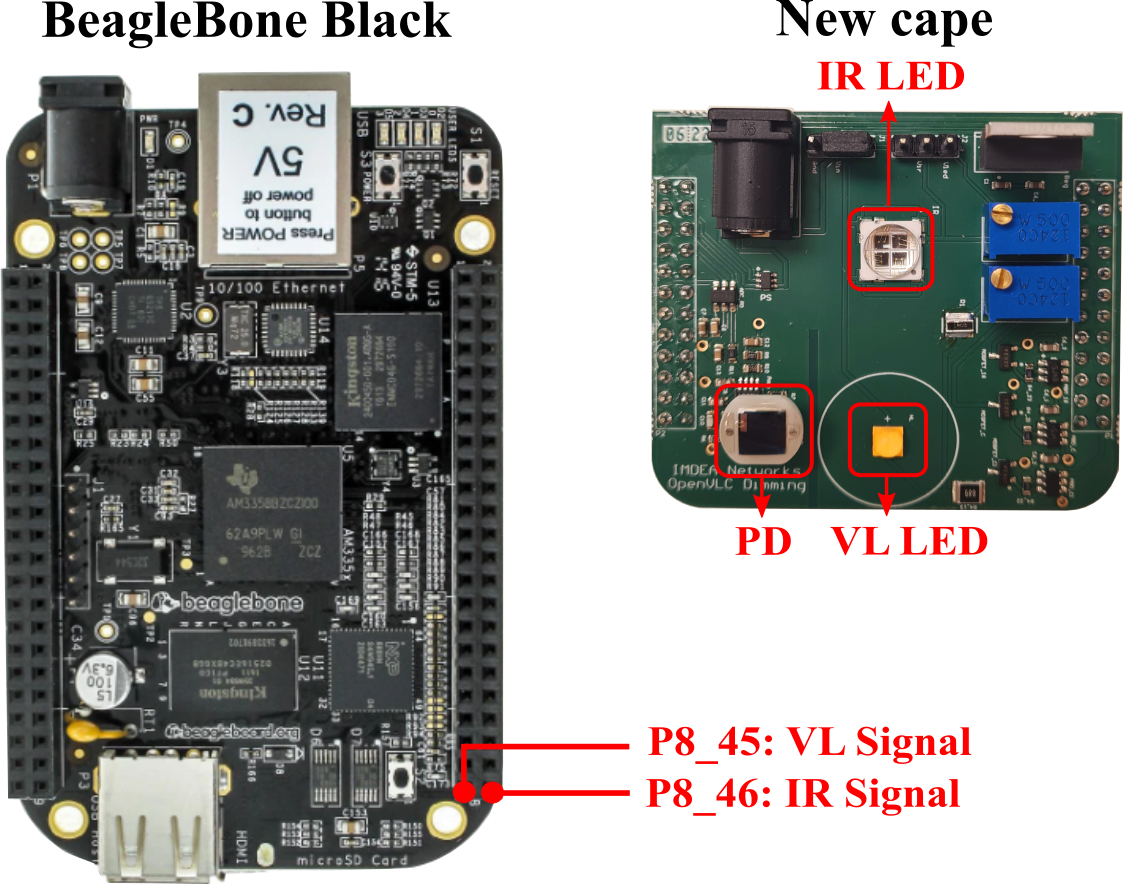
\includegraphics[width=0.9\columnwidth]{openvlc/Cape_for_TX_in_VL_IR_bands}
    \caption{Test iperf riportato nella documentazione di OpenVLC}
    \label{fig:beaglebone_cape}
\end{figure}

Durante la configurazione, sulle schede BeagleBone, viene installato il sistema operativo \textit{Debian 8 "jessie"}. Il driver di OpenVLC è di fatto un modulo del kernel \textit{Linux} che agisce da ponte tra lo stack di rete del sistema operativo e l'hardware BeagleBone.

\paragraph{Reti e Sicurezza.}
Una volta configurate correttamente due schede, la prima come trasmettitore e la seconda come ricevitore, è quindi possibile usarle come una \textit{common network interface}. Ovvero il sistema operativo, in questo caso Debian 8, può usare OpenVLC allo stesso modo in cui userebbe una normale interfaccia di rete, come ad esempio inviare/ricevere pacchetti IP e comunicare con altri dispositivi su una rete locale.\\
Come già anticipato, ognuna delle due schede ha uno ed un solo ruolo, non è infatti possibile attualmente trasmettere e ricevere dalla stessa scheda contemporaneamente. Questo tipo di canale di comunicazione viene denominato \textit{simplex} (unidirezionale), in contrapposizione ad esempio ad un canale \textit{duplex} in cui un device può cambiare ruolo dinamicamente o ad un canale \textit{full-duplex} in cui un device può trasmettere e ricevere simultaneamente.\\
In OpenVLC, per cambiare il ruolo di un device, bisogna di fatto ricompilare il driver.

OpenVLC, essendo un progetto di piccole dimensioni ed avendo come obbiettivo quello di sperimentare con la \gls{vlc}, piuttosto che usarla per comunicazioni realistiche, non implementa delle vere e proprie reti o un infrastruttura hardware/software che permetta di implementare delle reti di calcolatori.

Per quanto riguarda invece la sicurezza, il driver di OpenVLC, gestendo i livelli \gls{phy} e \gls{mac}, non implementa alcun meccanismo di sicurezza. Lascia invece che questa sia gestita dai livelli superiori. Tuttavia definire protocolli di sicurezza a livello fisico è decisamente utile, in particolar modo se si considera che la \gls{vlc} viene utilizzata in contesti in cui la sicurezza delle reti di comunicazione è critica, come ad esempio ospedali e convogli di veicoli.

In figura \ref{fig:design_openvlc} si riporta uno schema riassuntivo dell'architettura di OpenVLC in cui si può osservare quanto descritto precedentemente.
\begin{figure}[H] 
    \centering 
    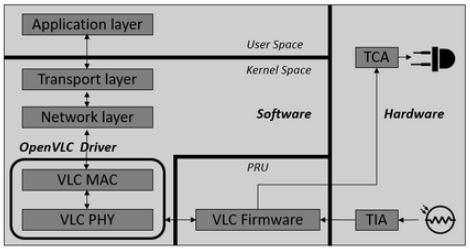
\includegraphics[width=0.9\columnwidth]{openvlc/design_openvlc}
    \caption{Architettura di OpenVLC (fonte: documentazione OpenVLC)}
    \label{fig:design_openvlc}
\end{figure}

\paragraph{PHY Frame.}

Come mostrato in figura \ref{fig:phy_frame_structure}, il \gls{phy} frame, cioè la struttura del pacchetto dati a livello fisico, si suddivide in diversi campi.\\
Ogni pacchetto inizia con un preambolo, lungo quattro byte, necessario alla sincronizzazione dei device, a cui segue lo \textit{Start of Frame Delimiter} che indica l'inizio del frame.\\
Successivamente vengono inviati quattro campi da due byte ciascuno: la lunghezza in byte del frame (\textit{Frame Length}), l'indirizzo del device a cui il pacchetto è destinato (\textit{Destination}), l'indirizzo del device da cui proviene (\textit{Source}) e il protocollo di comunicazione (\textit{Protocol}).
A questo punto sono presenti i dati veri e propri, contenuti nel \textit{Payload}, il quale ha una lunghezza variabile da 0 a 255 byte.
Infine, nel campo \textit{Error Correction Code}, si hanno 16 byte necessari alla correzione degli errori generati da Reed-Solomon.
\begin{figure}[H] 
    \centering 
    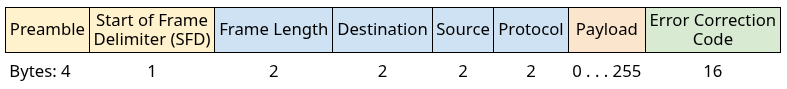
\includegraphics[width=0.9\columnwidth]{openvlc/phy_frame_structure}
    \caption{Struttura del PHY frame in OpenVLC}
    \label{fig:phy_frame_structure}
\end{figure}

\paragraph{Modulazione e Codifica.}
\noindent Come definito dallo standard \gls{ieee} 802.15.7, OpenVLC utilizza la modulazione \gls{ook}\glsfirstoccur nella trasmissione dei dati. In \gls{vlc}, la modulazione dei dati riguarda il modo in cui le informazioni digitali vengono convertite in un segnale analogico tramite la variazione dell'intensità luminosa. In pratica i dispositivi trasmettono bit mediante uno sfarfallio del LED impercettibile all'occhio umano. Si ricorda infatti che lo scopo primario del LED è l'illuminazione, di conseguenza è necessario che rimanga costantemente acceso e che questo sfarfallio sia impercettibile in modo tale da non essere fastidioso per gli occhi.\\
In \gls{vlc}, la modulazione \gls{ook}, è la forma più semplice di modulazione ASK (Amplitude Shift Keying), la quale rappresenta i dati digitali come presenza o assenza di un segnale luminoso che vengono interpretate rispettivamente come bit-1 e bit-0. Questa modulazione è facile da implementare ed ha un basso costo computazionale, tuttavia richiede una sincronizzazione molto precisa tra trasmettitore e ricevitore.

Al fianco della modulazione \gls{ook}, viene usata la codifica \textit{Manchester}, una forma di comunicazione dati nella quale ogni punto viene segnalato da una transizione. Ad esempio, la transizione del segnale, in questo caso luminoso, da basso ad alto viene interpretato dall scheda ricevente come bit-1; viceversa da alto a basso viene interpretato come un bit-0.\\
Nella \gls{vlc} ha il vantaggio di mantenere il bilanciamento DC, riducendo il rischio di \textit{flickering} (sfarfallio) visibile e migliora la sincronizzazione tra trasmettitore e ricevitore.
In OpenVLC l'unico campo del \gls{phy} frame in cui non viene applicata la codifica Manchester è il preambolo, che di conseguenza viene trasmesso in semplice \gls{ook}.

\paragraph{Correzione degli Errori.}
In OpenVLC, la correzione degli errori è gestita tramite i codici Reed-Solomon, ovvero codici di correzione degli errori applicati a livello fisico nella \gls{vlc} per migliorare l'affidabilità della comunicazione e compensare gli errori introdotti da disturbi ambientali.\\
Sia k il numero di byte informativi ed n il numero di byte totali trasmessi, Reed-Solomon RS(n,k) è in grado di correggere fino a (n-k)/2 byte errati.

Nel caso di OpenVLC viene usato RS(216,200), di conseguenza vengono aggiunti 16 byte di correzione degli errori per 200 byte informativi. RS(216,200) non possiede una grandissima capacità di correzione degli errori, ma essendo OpenVLC orientato alla velocità piuttosto che all'affidabilità, riduce sicuramente latenza ed overhead rispetto a varianti di Reed-Solomon più performanti.

\paragraph{Configurazione.}
I dettagli su come è stato configurato il sistema in questo progetto, sulle problematiche riscontrate e su come sono state risolte, si possono trovare nell'appendice \ref{app:A}.


% ================================================================= %
\section{Vulnerabilità}

% cosa assumi sull'attaccante: posizione buona per intercettare il fascio, rubare i pacchet-
% ti, rubare le password, modificare pacchetti, distruggere pacchetti a caso o mandare
% pacchetti a caso

% possibili attacchi e Vulnerabilità
Di seguito vengono elencate le principali vulnerabilità individuate della \gls{vlc}, ed in particolare di OpenVLC, che come menzionato precedentemente non presenta alcun meccanismo di sicurezza, essendo una piattaforma sperimentale ed orientata alla velocità.\\
Queste vulnerabilità sono particolarmente rilevanti in contesti in cui la sicurezza della rete è critica, come ambienti industriali, ospedalieri o automotive.

\begin{itemize}
    % risolvibili da authentication
    \item \textbf{Injection di pacchetti.} In assenza di autenticazione, un dispositivo non autorizzato può trasmettere pacchetti arbitrari sulla rete VLC, simulando il comportamento di un nodo legittimo e causando malfunzionamenti o attacchi di spoofing.
    \item \textbf{Replay di messaggi.} Senza meccanismi di autenticazione e protezione, è possibile catturare e ritrasmettere pacchetti validi, inducendo il ricevitore ad accettare messaggi duplicati o obsoleti.
    % risolvibile da integrity (MIC)
    \item \textbf{Man-in-the-Middle (MitM).} Un attaccante può inserirsi tra trasmettitore e ricevitore, modificando i pacchetti in transito o iniettando messaggi malevoli, compromettendo l'integrità e l'autenticità della comunicazione.
    % risolvibile da confidentiality
    \item \textbf{Intercettazione del segnale ottico.} Un attaccante posizionato in modo opportuno può intercettare il fascio luminoso trasmesso tra i dispositivi, acquisendo i pacchetti scambiati e potenzialmente informazioni sensibili come password o dati privati. Come si osserverà dai risultati dei test nel capitolo \ref{cap:test}, considerando che la luce visibile non si propaga in maniera totalmente unidirezionale, questo tipo di attacco non è una possibilità remota, nel momento in cui l'attaccante ha accesso all'ambiente in cui avviene la comunicazione.
    % irrisolvibile se l'attaccante ha accesso al luogo della comunicazione, oppure con codici di correzione molto potenti
    \item \textbf{Distruzione o alterazione dei pacchetti.} Un attaccante può disturbare la comunicazione inviando segnali ottici che interferiscono con la trasmissione, causando la perdita o la corruzione dei dati.
\end{itemize}

\subsection{Principi di crittografia e limitazioni}
Prima di poter parlare della soluzione proposta è necessario specificare che l'autenticazione è solo uno dei pilastri della sicurezza dell'informazione. Infatti, per garantire la robustezza del sistema da tutti questi possibili attacchi, è indispensabile affiancare all'autenticazione la confidenzialità, l'integrità e la correzione degli errori.

L'autenticazione infatti garantisce l'identità del mittente di un messaggio, ma non impedisce a terzi di leggere il contenuto del messaggio. Questo si può ottenere però dalla confidenzialità, grazie alla quale solo il destinatario è in grado di decifrare e leggere il messaggio.\\
Allo stesso modo, non garantisce che il messaggio non sia manipolato in modo tale da risultare proveniente dallo stesso mittente, ma con un contenuto diverso dall'originale. Implementare dei meccanismi di integrità garantisce al destinatario che il messaggio non sia stato manipolato in alcun modo.\\
Parallelamente, la correzione degli errori garantisce una maggio resilienza nel caso in cui l'attaccante voglia solo disturbare la comunicazione.

Nella pratica, la soluzione più comune è la crittografia simmetrica. Secondo questa tecnica di cifratura dei messaggi, prima della comunicazione i due device si scambiano una chiave condivisa attraverso un canale sicuro, e usano questa chiave per cifrare i messaggi. In questo modo la crittografia simmetrica garantisce simultaneamente autenticazione e confidenzialità.

Ovviamente ad un aumento della sicurezza, corrispondono inevitabilmente rallentamenti nella comunicazione, in quanto è necessaria una maggiore elaborazione dei dati. Pertanto, bisogna contestualizzare e comprendere le reali necessità del sistema per bilanciare questo \textit{trade-off}.

% ================================================================= %
\section{Soluzione proposta}

Per far fronte a tali Vulnerabilità, la soluzione che si propone è l'autenticazione a livello fisico dei messaggi. L'idea di fondo è di fare in modo che il device trasmettitore incorpori nei suoi segnali fisici una \gls{otp} derivata da una \gls{psk}. Il device ricevitore rileva tale \gls{otp}, la estrae dai segnali fisici e la verifica, autenticando, se risulta valida, il device trasmettitore. Se invece non viene rilevata una \gls{otp} valida, il pacchetto viene scartato prima di ulteriori elaborazioni.

La \gls{psk} è una chiave segreta condivisa tra i due dispositivi prima dell'inizio della comunicazione. Può essere condivisa attraverso un canale di comunicazione sicuro, oppure, come nel caso di questo progetto, può essere \textit{"hard-coded"}, cioè codificata direttamente nel codice sorgente dei dispositivi.


\paragraph{Vulnerabilità Contrastate dall'Autenticazione.}

L'autenticazione sviluppata in questo progetto è volta a risolvere un sottoinsieme delle vulnerabilità sopra elencate, in particolare injection di pacchetti e replay dei messaggi.

Nell'injection di pacchetti, l'attaccante si finge un nodo legittimo della rete e mette in circolazione pacchetti aventi un contenuto malevolo o semplicemente volti a congestionarla deteriorando così la qualità della comunicazione e le risorse degli altri dispositivi. Questo tipo di attacco può essere prevenuto dall'autenticazione a livello fisico, in quanto ogni pacchetto che non possiede una \gls{otp} valida, come ad esempio quelli forgiati dall'attaccante (che si suppone non abbia la \gls{psk} necessaria a generare una \gls{otp} valida), viene prontamente scartato, evitando ulteriori elaborazioni che possanno depletare le risorse del device o addirittura eseguire codice malevolo. Anche nel caso in cui l'attaccante abbia il pieno controllo di un nodo legittimo (e di conseguenza anche alla \gls{psk} e alla generazione di \gls{otp} valide), e quindi sia in grado di superare i controlli a livello fisico, il coordinatore della rete, dato che la \gls{otp} è device-specifica, può risalire al nodo corrotto leggendo la \gls{otp} dei pacchetti malevoli e contrassegnarlo come illegittimo.

Nel replay dei messaggi, l'attaccante cattura messaggi legittimi inviati da un nodo della rete e, senza modificarli, li ritrasmette in modo tale da congestionare la rete e depletare le risorse del sistema. Anche questo tipo di attacco può essere prevenuto dall'autenticazione sviluppata, poiché, per come è stato progettato l'algoritmo di generazione della \gls{otp}, ogni \gls{otp} (e di riflesso ogni pacchetto) è valida per un unico utilizzo. Quindi una volta trasmesso un pacchetto replicato, se trasmesso una seconda volta, questo verrà scartato dal device ricevitore in quanto la \gls{otp} in esso contenuta risulterà scaduta.


\paragraph{Possibili Contromisure alle altre Vulnerabilità.}
Una possibile contromisura all'attacco Man-in-the-Middle si può implementare semplicemente aggiungendo un \gls{mic} al \gls{phy} frame. Ovvero un codice generato da una funzione di hash, calcolato sia sulla \gls{otp} che sul payload, che possa essere verificato dal ricevitore, in modo tale da assicurare che il messaggio non abbia ricevuto modifiche non autorizzate durante la trasmissione.

L'intercettazione del segnale ottico si può mitigare attraverso la crittografia dei messaggi, ad esempio criptando il messaggio con la chiave pubblica del device destinatario, in modo tale che sia l'unico in grado di decifrarlo e leggerne il contenuto. Oppure usando una chiave condivisa tra i due device in modo tale da garantire al contempo anche l'autenticazione.

L'ultima vulnerabilità, cioè la distruzione o alterazione dei pacchetti tramite segnali ottici che interferiscono con la comunicazione, è in realtà già mitigata attraverso i codici di correzione degli errori presenti in OpenVLC (Reed-Solomon), tuttavia si potrebbe pensare di implementare delle varianti capaci di correggere un maggior numero di errori, anche se al costo di rallentare la comunicazione.